% !TEX encoding = UTF-8
% !TEX TS-program = pdflatex
% !TEX root = ../tesi.tex


\chapter{L'Azienda}
\label{cap1:L'Azienda}
%**************************************************************

%Introduzione al contesto applicativo.\\

%\noindent Esempio di utilizzo di un termine nel glossario \\
%\gls{api}. \\

%\noindent Esempio di citazione in linea \\
%\cite{site:agile-manifesto}. \\

%\noindent Esempio di citazione nel pie' di pagina \\
%citazione\footcite{womak:lean-thinking} \\

%**************************************************************

\textit{Questo capitolo descrive nel dettaglio l'azienda ospitante andando a definire il suo business, l’organizzazione interna e le tecnologie adottate per soddisfare i clienti.}

\section{Presentazione dell'azienda}
\label{cap1:Presentazione dell'azienda}
Questa sezione si concentra sull'azienda che ha ospitato lo stage, fornendo una chiara spiegazione dei prodotti e servizi forniti assieme alla descrizione delle tecnologie adottate.

\subsection{\azienda}
\label{cap1:Tepui}
\paragraph*{}\azienda\ è una software house specializzata nello sviluppo di applicazioni gestionali attraverso l'utilizzo di strumenti CASE. 

\paragraph*{}Nasce nel 2016 dall'idea di tre persone. I fondatori hanno incontrato diverse realtà lavorative prima di portare avanti il progetto di aprire un'azienda. Due di queste persone hanno lavorato nell'ambito della business intelligence. Loro hanno riscontrato che è molto difficile analizzare i dati delle aziende in quanto ognuna di esse è diversa dalle altre, soprattutto nella gestione dei database o data warehouse. Sono arrivati alla conclusione che, se fosse possibile fornire un prodotto software standardizzato, sarebbe molto più semplice anche l'analisi dei loro dati. Quindi i due hanno iniziato a cercare un'applicazione che permettesse di creare software in maniera rapida e compatibile con diversi sistemi operativi. Il risultato della loro ricerca è stato \inde\ e hanno così conosciuto il terzo fondatore già esperto dell'applicazione che li ha formati nel suo utilizzo.

\begin{figure}[!h] 
	\centering 
	
\includegraphics[width=0.5\columnwidth]{logo-tepui} 
	\caption{Logo dell'azienda}
\end{figure}

 
\paragraph*{}I tre fondatori sono fortemente convinti nei vantaggi tecnologici ed economici che l'implementazione mediante strumenti di sviluppo rapido porta ai propri clienti. Agli inizi l'azienda si è dedicata alla creazione di software e mantenimento di applicazioni già presenti nel mercato realizzate con \inde. Dopo un anno, raggiunta una certa stabilità e un buon numero di clienti, si è evoluta ed ha iniziato ad esplorare l'ambito della business intelligence affidandosi a Yallpa S.r.l, oggi partner strategico. 

 
%Prima della nascita di \azienda\, bisogna parlare di Yallpa S.r.l. Questa azienda nasceva  è nata Yallpa s.r.l., una azienda dedita alla Business Intelligence. L'azienda in questione procedeva alle sue analisi adottando Access, Microsoft SQL Server e non elargiva alcun software per la gestione dei dati. Due impiegati si sono accorti che offrire un prodotto costruito con un certo criterio può facilitare notevolmente la Business Intelligence, così è iniziato un movimento alla ricerca di un'applicazione che permettesse la creazione di applicazioni gestionali e si è arrivati a \inde. 

%\paragraph*{}Nel 2016 nasce, dall'unione delle idee dei due impiegati e un terzo membro già esperto di \inde\, l'azienda \azienda\ . I tre fondatori erano e sono ad oggi convinti fortemente nei vantaggi tecnologici ed economici che l'implementazione mediante strumenti di sviluppo rapido porta ai propri clienti. All'inizio tuttavia la Business Intelligence è stata messa da parte per dedicarsi alla realizzazione di software con \inde\ . Dopo un anno, raggiunta una certa stabilità e un buon numero di clienti, si è evoluta ed ha iniziato ad esplorare l'ambito della Business Intelligence affidandosi a Yallpa S.r.l, oggi partner strategico dell'azienda. 

\paragraph*{}L'azienda opera principalmente a livello nazionale con sedi in Veneto e Lombardia. Essa propone soluzioni a pacchetto e/o realizzate da specifiche richieste del cliente. Per la realizzazione delle applicazioni, lo strumento che viene adottato maggiormente è \inde\.
Oltre allo sviluppo di software, l'azienda si occupa anche di data warehousing e business intelligence attraverso la suite dei prodotti Qlik e Microsoft Power BI.


\subsection{Prodotti e servizi}
\label{cap1:Prodotti e servizi}
I principali prodotti realizzati dall'azienda sono i software gestionali. Essi rappresentano l'insieme dei software che automatizzano i processi di gestione all'interno delle aziende. Si dividono principalmente nei seguenti macro gruppi:
\begin{itemize}
	\item Software di contabilità;
	\item Software per il magazzino;
	\item Software per la produzione;
	\item Software per il budgeting;
	\item Software di gestione ed analisi finanziaria;
	\item Software dedicato.
\end{itemize}

\begin{figure}[!h] 
	\centering 
	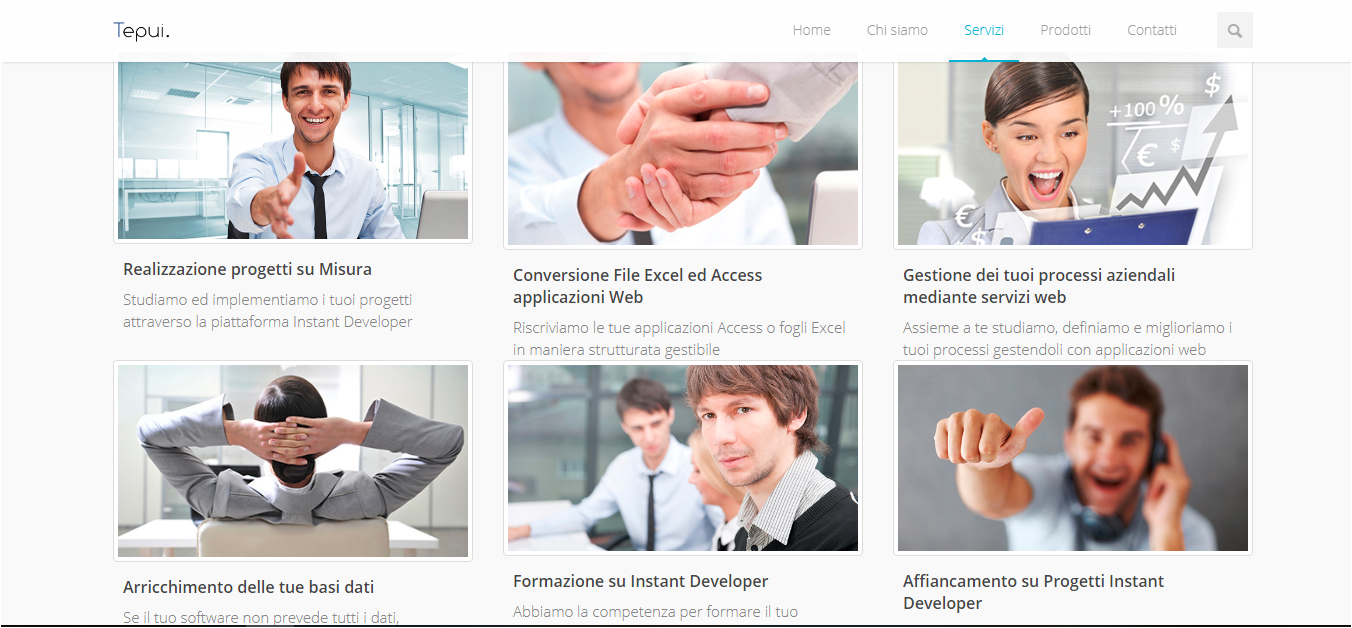
\includegraphics[width=0.8\columnwidth]{immagineServizi} 
	\caption{Prodotti e servizi forniti nella loro pagina web}
\end{figure}

\azienda\ persegue due diverse soluzioni per la creazione dei prodotti software: a pacchetto e su misura. Le soluzioni a pacchetto consistono in software completi già disponibili all'interno dell'azienda destinati alla vendita. Tuttavia, la loro vendita non è immediata ma segue comunque un controllo e modifica per adattare il prodotto venduto alla realtà del cliente. L'altro tipo di soluzione consiste, invece, nella realizzazione da zero di un prodotto. Questo tipo di servizio prevede tutti i passaggi dallo studio del problema alla realizzazione del prodotto completo.

Infine, in merito ai servizi, viene fornito la manutenzione di un qualsiasi prodotto \inde, sia esso creato da \azienda\ o da una qualsiasi altra ditta che fa affidamento a tale piattaforma, purché si disponga del codice sorgente. Inoltre, tra i servizi troviamo anche: formazione su \inde, affiancamento ai progetti con \inde, conversione dei file Excel ed Access in applicazioni web e la possibilità di sfruttare prodotti web per i processi aziendali.


\subsection{Tecnologie di riferimento}
\label{cap1:Tecnologie di riferimento}
\subsubsection*{Linguaggi di programmazione}

L'azienda opera nell'ambito web. I prodotti realizzati si basano sui seguenti linguaggi di programmazione lato server: 
\begin{itemize}
	\item \textbf{C\#}: linguaggio di programmazione orientato agli oggetti che consente di creare una vasta gamma di applicazioni protette e affidabili per .NET Framework. Esso può essere adottato per creare applicazioni client Windows, servizi Web XML, componenti distribuiti, applicazioni client\-server, applicazioni di database e molto altro.
	
	\item \textbf{Java}: linguaggio di programmazione ad alto livello, orientato agli oggetti e a tipizzazione statica, che si appoggia sull'omonima piattaforma software, specificamente progettato per essere il più possibile indipendente dalla piattaforma hardware di esecuzione.
\end{itemize}

Per quanto riguarda la componente grafica, le tecnologie adottate sono: HTML5, CSS3 e Javascript.

\begin{figure}[!h] 
	\centering 
	\includegraphics[width=0.8\columnwidth]{Tecnologie} 
	\caption{Linguaggi di programmazione}
\end{figure}

\subsubsection*{Database}
Tutte le applicazioni dell'azienda mirano alla realizzazione di software gestionale, i quali necessitano di uno o più database, o per realtà più grandi dei Data Warehouse. I principali  database che hanno avuto modo di incontrare nello svolgimento delle loro attività sono stati: MySql, DB2, PostgreSQL, Oracle e SQL Server.\\

Tra i differenti database disponibili, quello adottato dall'azienda è SQL Server. La scelta ricade su questo dispositivo perché rappresenta un punto di incontro tra prestazioni e costi contenuti, ma anche per il suo elevato utilizzo da parte delle aziende del territorio e per la sua popolarità visto che ancora oggi risulta essere il terzo database più usato al mondo dopo Oracle e MySQL. 

\begin{figure}[!h] 
	\centering 
	
\includegraphics[width=0.8\columnwidth]{database} 
	\caption{Database}
\end{figure}


\section{Processi aziendali}
\label{cap1:Processi aziendali}

Questa sezione presenta l'organizzazione dell'azienda e come quest'ultima cerchi di migliorarsi nel corso del tempo. 

\subsection{Miglioramento della qualità dei processi}
\label{cap1:Miglioramento della qualità dei processi}

\azienda nello svolgimento delle proprie attività opta per perseguire il costante miglioramento dei processi. Per fare questo fa affidamento al ciclo PDCA che si compone di quattro attività:
\begin{itemize}
	\item \textbf{P}lan: individuazione degli obiettivi di miglioramento e creazione di un piano d'azione nello svolgimento dei lavori;
	\item \textbf{D}o: esecuzione di quanto pianificato;
	\item \textbf{C}heck: analisi dei risultati ottenuti nella fase precedente e confronto con quanto pianificato; 
	\item \textbf{A}ct: standardizzazione delle attività andate a buon fine e rielaborazione di quelle da migliorare ricominciando con la pianificazione.
\end{itemize}

\begin{figure}[!h] 
	\centering 
	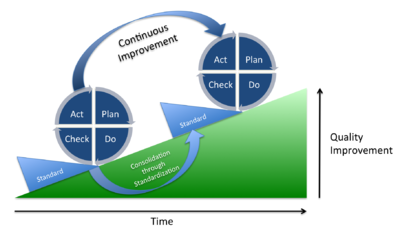
\includegraphics[width=0.8\columnwidth]{PDCA} 
	\caption{Ciclo PDCA}
\end{figure}

Durante lo stage, ho notato che l'azienda adotta questa strategia principalmente nel processo di sviluppo mirando ad ottenere un prodotto efficiente ed efficacie. Negli altri processi aziendali invece, quale ad esempio la documentazione, è ancora in fase di sviluppo. La documentazione realizzata non è sempre completa. Viene preferito affidarsi ai mock\-up ed ai documenti che descrivono le caratteristiche tecniche e grafiche del prodotto in maniera poco completa. Quando l'ideale sarebbe indagare su questi punti, ma in maniera più dettagliata fin dall'inizio. Infatti, nel corso del progetto mi sono trovato diverse volte a chiedere informazioni al tutor aziendale (responsabile di progetto), in merito a delle funzionalità non espresse nei documenti redatti e a me consegnati.  

\subsection{Metodologia agile}
\label{cap1:Metodologia agile}

L'azienda nello sviluppo delle applicazioni adotta la metodologia agile. Questo metodo operativo permette una maggiore libertà rispetto ad altri tipi quali sequenziale, incrementale o a spirale. I punti fondamentali sono:
\begin{itemize}
	\item privilegiare la realizzazione del software alla creazione di documentazione;
	\item collaborare con il cliente invece di dedicarsi a contrattazioni;
	\item essere pronti a reagire ad ogni situazione invece di avere un piano di gestione dei rischi.
\end{itemize}
\azienda\ ha deciso di adottare questo metodo lavorativo per i sui prodotti perché hanno osservato come nella realtà lavorativa le aziende vorrebbero avere a disposizione prodotti efficienti ed efficaci in tempi molto brevi. 
Inoltre, la scelta è ricaduta su questa tipologia per un motivo molto importante secondo l'azienda: conoscere i clienti, il mercato e creare un rapporto duraturo di fiducia. 

Questo metodo si concretizza con degli incontri la cui scadenza è variabile, settimanale, bisettimanale o mensili, con i clienti. Durante gli incontri si raccolgono task, migliorie da apportare ai progetti o addirittura ci si ferma dal cliente per realizzare nuove funzionalità e chiedere informazioni in maniera immediata. Così facendo la comunicazione è rapida, le mail sono ridotte ed è molto più facile comprendere le necessità delle aziende cliente osservandola dall'intero.


\section{Strumenti a supporto dei processi}
\label{cap1:Strumenti a supporto dei processi}

Questa sezione illustra quali strumenti vengono adoperati a supporto dei processi e per lo sviluppo mirati a garantire qualità dei prodotti e servizi.

\subsection{Gestione di progetto}
\label{cap1:Gestione di progetto}

La gestione di progetto consiste nel definire ed organizzare il lavoro da svolgere in tempi e modi ben definiti. Per tale processo vengono utilizzati tre strumenti: Microsoft Teams, iDo e le mail.

\paragraph{Micorsoft Teams} è un'applicazione di telecomunicazione nel quale possono essere creati diversi gruppi con all'interno molti canali di comunicazione ai quali possono accedere solo le persone invitate. L'azienda crea un gruppo per ogni azienda e all'interno prevede un canale generale dove inserire documentazione o fare domande di natura generica, mentre gli altri riguardano un progetto specifico o le singole funzionalità da implementare, se vi è un unico progetto. 

\begin{figure}[!h] 
	\centering 
	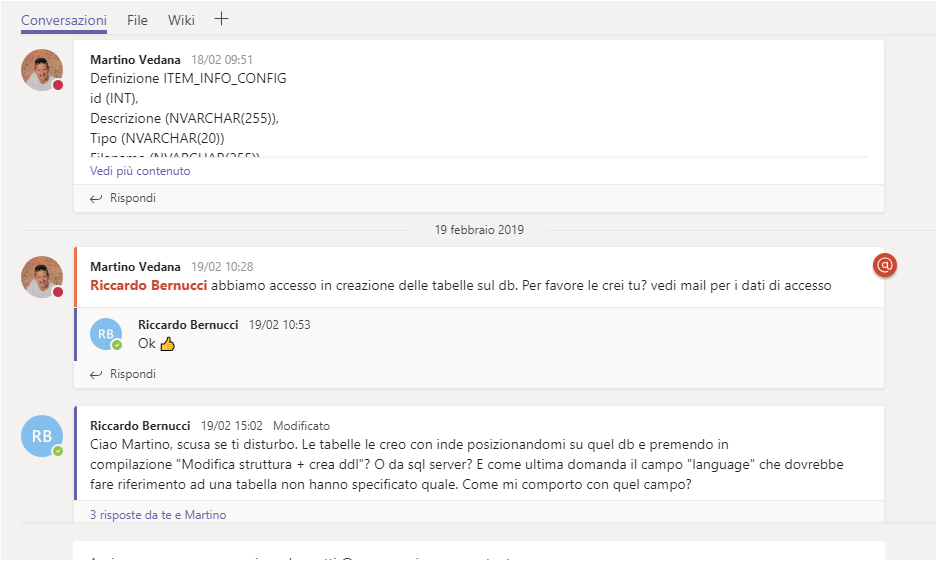
\includegraphics[height=0.4\columnwidth]{Teams} 
	\caption{Conversazione su Teams}
\end{figure}


\paragraph{Mail} ovvero la posta elettronica. Per iniziare il progetto mi è stata fornita una mail aziendale. Le mail servono per comunicare in maniera tempestiva la creazione ed assegnazione di una commessa nell'applicazione iDo. Queste ultime sono il principale mezzo di comunicazione con le aziende clienti. Una prassi interna all'azienda è che per informazioni da chiedere al cliente, bisogna prima discuterne internamente tra i membri del gruppo assegnato a quel progetto e poi quella di mettere in copia carbone il responsabile di progetto alla eventuale mail da inviare ai clienti.



\paragraph{iDo} è un'applicazione web realizzata con \inde dove vengono assegnate le commesse, indicando tempi di inizio e fine previsti. In questo applicativo, si devono indicare le ore svolte dai lavoratori specificando le ore di inizio, fine e informazioni di quanto si è svolto in quel periodo. Inoltre, si possono inserire commenti utili all'azienda cliente e a \azienda. 
Grazie a questa applicazione viene calcolato il compenso e il consuntivo del progetto. Essa si compone di diverse sezioni la Kanban (\hyperref[ido]{figura \ref{ido}}), dove vengono presentate tutte le commesse con in testa il nome del cliente e del progetto; una sezione Commessa, nella quale vengono inseriti i progetti assegnati e navigando al suo interno si accede alle commesse; una sezione tempi, dedicata a sistemare eventuali errori di inserimento a fine mese o per controllare le attività svolte dai dipendenti e prendere le opportune decisioni.

\begin{figure}[!h] 
	\centering 
	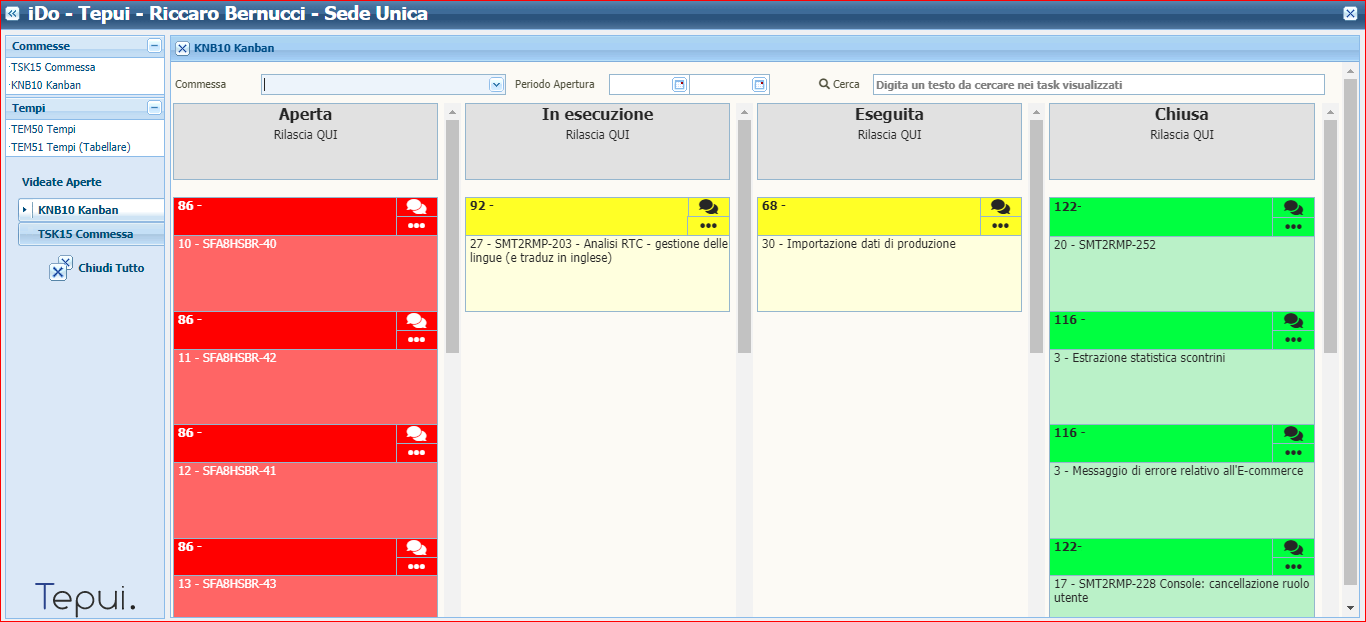
\includegraphics[width=0.8\columnwidth]{iDo} 
	\caption{Kanban dell'applicazione iDo (con nome cliente censurato)}
	\label{ido}
\end{figure}



\subsection{Documentazione}
\label{cap1:Documentazione}

L'azienda sebbene abbia deciso di adottare un modello agile non è priva di documenti. Quando deve realizzare un progetto il primo passo è quello di redigere un Piano di progetto e POC documentale con le principali caratteristiche che il prodotto finale dovrà avere. 
Il motivo per cui l'azienda dà molta importanza al POC è che, con un documento nel quale è riportato la struttura del database e la grafica pressapochista che il progetto dovrà avere, permette di realizzare un prodotto completo in 3/4 settimane. 
La documentazione è tenuta interamente su OneDrive For Business. Ogni documento ha una sua collocazione da rispettare. 

\subsection{Sistema di versionamento}
\label{cap1:Sistema di versionamento}

Per il versionamento e il salvataggio dei File prodotti durante la realizzazione dei progetti è previsto l'utilizzo di una repository creata dal Project Manager su un'applicazione basata sempre su InDe, TeamWorks. Successivamente, vengono forniti ai dipendenti scelti nella realizzazione di uno specifico progetto i permessi di: scrittura, lettura ed eliminazione.
Tale applicazione web risulta essere molto simile a GitHub, tuttavia è molto più intuitivo e semplice perché le funzionalità permesse sono controllare informazioni relative ai commit, tornare indietro di versione (rollback), scaricare progetti (Download) e creare dei derivati (Fork) premendo unicamente dei pulsanti.

Ciascun progetto deve essere soggetto a versionamento perciò chiunque lo utilizza ha una visione chiara e dettagliata della sua storia e delle sue modifche. Ad ogni task deve corrispondere una versione. Nelle versioni viene applicato il segeunte formalismo:
\begin{center}
	X.Y.Z
\end{center}
Dove X,Y,Z sono numeri incrementali da 0 a infinito. 
Z indica i singoli task e bug individuati ed risolti, Y rappresenta la implementazione di nuove funzionalità rilasciate per la fase di collaudo e X quando il progetto ha superato il collaudo e diventa operativo.  

\subsubsection{Sistema di pubblicazione}
La pubblicazione presso \azienda\ corrisponde al rilascio dell'applicazione all'azienda cliente per effettuare dei test. Il collaudo viene effettuato anche internamente all'azienda, ma questa doppio controllo permette di realizzare applicazioni corrette che non necessitino di eccessive manutenzioni di tipo correttivo. 
Il sistema adottato dall'azienda per pubblicare il software è IDManager, anche essa una applicazione web di InDe, la quale permette di modificare i riferimenti del database cambiando la stringa di connessione del progetto e permette di caricare unicamente le differenze tra la versione precedente e quella attuale.


\subsection{Ambiente di sviluppo}
\label{cap1:Ambiente di sviluppo}

\paragraph{\inde} \'E l'ambiente di sviluppo adottato dell'azienda. Consiste in una piattaforma ad alta produttività, per lo sviluppo di applicazioni cross-platform (Web-based) creata da Pro Gamma S.p.A.. La scelta dell'azienda ricade su questo tipo di strumento per i seguenti vantaggi:
\begin{itemize}
	\item Scrivere l'applicazione e poterla distribuire in ambiente Java o Microsoft C\#;
	\item Collegare ed utilizzare più database contemporaneamente anche di tipo differente;
	\item Implementare applicazioni Desktop e Mobile;
	\item Gestire i rilasci successivi in maniera sicura e strutturata;
	\item Potersi focalizzare sui processi da gestire, sui i dati da memorizzare o modificare, evitando di dover programmare a basso livello, avendo però la possibilità, quando necessario, di poterlo fare.
\end{itemize}
Le applicazioni prodotte sono perciò nativamente multi-piattaforma, cross-browser, multi-database già nel momento in cui vengono create.

\paragraph{Microsoft SQL Server} Un DBMS relazionale, prodotto da Microsoft, che usa T-SQL, una variante del linguaggio SQL Standard. 

\paragraph{Microsoft SQL Server Management Studio 2017} \'E un'applicazione software che viene utilizzata per la configurazione, la gestione e l'amministrazione di tutti i componenti all'interno di Microsoft SQL Server. Lo strumento include sia editor di script che strumenti grafici che funzionano con oggetti e funzionalità del server.

\paragraph{Qlik}\'E un pacchetto che offre QlikView, Qlik Sense ed NPrinting. Essi sono software di visualizzazione e business intelligence che permettono il rapido sviluppo di dashboard completamente personalizzabili in grado di fornire rapidamente informazioni utili sui dati a disposizione.

\paragraph{Microsoft Power BI}
\'E un servizio di analisi aziendale di Microsoft. Mira a fornire visualizzazioni interattive e funzionalità di business intelligence con un'interfaccia abbastanza semplice da consentire agli utenti finali di creare i propri report e dashboard.

\subsubsection*{Altri strumenti}
Oltre agli strumenti appena descritti, eventuali IDE per scrivere in C\#, Java e gli altri linguaggi riportati in Sezione \ref{cap1:Tecnologie di riferimento}, sono lasciati al programmatore. Può capitare che nel corso di un progetto siano richieste  modifiche specifiche che l'applicazione \inde\ non permette, in quei casi vi è una modalità di inserimento personalizzato che consente di scrivere codice.



\subsection{Sistemi operativi}
\label{cap1:Sistemi operativi}

L'azienda usa  solo i sistemi operativi di Windows. Questo perché risultano essere gli unici compatibili con \inde. Per chi non dovesse avere a disposizione tale sistema operativo viene fornita una macchina virtuale alla quale collegarsi. 

\subsubsection*{VPN e desktop remoto}
In base al progetto, spesso può capitare che ci si debba affidare alla macchina virtuale del cliente. In queste occasioni l'azienda consiglia l'utilizzo di una delle seguenti applicazioni per connettersi alla VPN: openVPN, FortiClient o lo strumento di Windows. 
Mentre per entrare in desktop remoto: Connessione Desktop Remoto di windows oppure nRemoteNG, il quale offre anche la possibilità di creare una o più connessione VPN ed aprire diversi schermi remoti contemporaneamente. 
Quando invece si effettuano delle assistenze, AnyDesk o TeamViewer sono dei software efficienti per collegarsi al desktop del cliente e risolvere problemi.


\section{Clientela}
\label{cap1:Clientela}
I clienti di \azienda\ risiedono nei territori del nord Italia. La sede legale dell'azienda è a Milano, mentre a Castelfranco Veneto vi è la sede operativa che ha ospitato lo stage. I clienti dell'azienda sono imprese di medio-grandi dimensioni. Degne di nota troviamo Aton s.p.a, Sistemi s.p.a, WiseEnergy Italia s.r.l ed altre aziende che operano a livello internazionale.

\paragraph*{}In seguito alla compilazione dell'\hyperref[NDA]{Accordo di non divulgazione} per l'intera durata del progetto non verrà nominato il nome dell'azienda cliente.

\newpage